\documentclass[tikz,border=10pt]{standalone}
\usepackage{tikz}
\usetikzlibrary{positioning, calc, arrows.meta} % modern arrows

\begin{document}
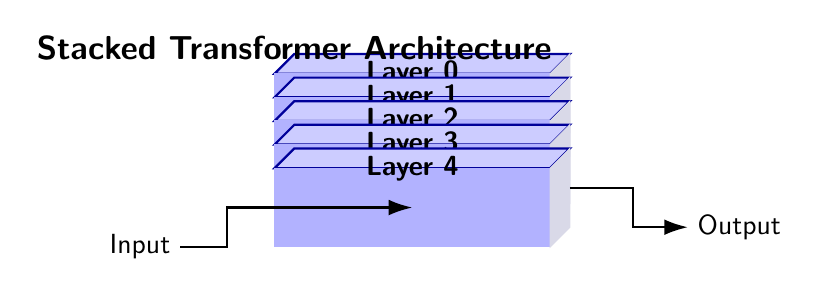
\begin{tikzpicture}[
    layerstyle/.style={
        draw=blue!60!black,
        fill=blue!20,
        line width=0.8pt
    },
    arrow/.style={
        -{Latex[length=3mm, width=2mm]},
        thick
    },
    font=\sffamily
]

% parameters
\def\w{3.5}
\def\h{1.0}
\def\d{0.25}

% macro: draw one "3D" layer
\newcommand{\drawlayer}[3]{
  \coordinate (A) at (#1,#2);
  \coordinate (B) at ($(A)+(\w,0)$);
  \coordinate (C) at ($(B)+(\d,\d)$);
  \coordinate (D) at ($(A)+(\d,\d)$);
  \coordinate (E) at ($(A)+(0,\h)$);
  \coordinate (F) at ($(E)+(\w,0)$);
  \coordinate (G) at ($(F)+(\d,\d)$);
  \coordinate (H) at ($(E)+(\d,\d)$);

  \filldraw[layerstyle] (E) -- (F) -- (G) -- (H) -- cycle; % top
  \filldraw[blue!30!white] (A) -- (B) -- (F) -- (E) -- cycle; % front
  \filldraw[blue!40!black!15] (B) -- (C) -- (G) -- (F) -- cycle; % side
  \node[font=\sffamily\bfseries, align=center] at ($(A)!0.5!(F)+(0,0.5*\h)$) {#3};
}

% draw 5 stacked layers
\foreach \i in {0,...,4}{
  \pgfmathsetmacro{\y}{-\i*0.3}
  \drawlayer{0}{\y}{Layer \i};
}

% arrows and labels
\node[font=\sffamily, left=1.2cm of A] (input) {Input};
\draw[arrow] (input.east) -- ++(0.6,0) |- ($(A)!0.5!(F)$);

\node[font=\sffamily, right=1.5cm of C] (output) {Output};
\draw[arrow] ($(C)!0.5!(G)$) -- ++(0.8,0) |- (output.west);

\node[font=\sffamily\large\bfseries, above=1cm of H] {Stacked Transformer Architecture};

\end{tikzpicture}
\end{document}

